\subchapter{Lab1: Building and Booting a Preempt-RT Kernel}{Download, Configure, Build and Boot}

During this lab, you will:
\begin{itemize}
	\item Configure the Buildroot Build-system to generate an image based on the upstream linux-rt repository
	\item Configure the kernel to enable full preemption
	\item Boot the system and check that it runs preempt-rt
\end{itemize}

\section{Initial Setup}
As specified in the Buildroot
manual\footnote{\url{https://buildroot.org/downloads/manual/manual.html\#requirement-mandatory}},
Buildroot requires a few packages to be installed on your
machine. Let's install them using Ubuntu's package manager:

\begin{bashinput}
sudo apt install sed make binutils gcc g++ bash patch \
  gzip bzip2 perl tar cpio python unzip rsync wget libncurses-dev
\end{bashinput}

\section{Download Buildroot}

Since we're going to do Buildroot development, let's clone the
Buildroot source code from its Git repository:

\begin{bashinput}
git clone git://git.busybox.net/buildroot
\end{bashinput}

In case this is blocked on your network, you can download the Buildroot
tarball \code{buildroot-2021.11.tar.bz2} from
\code{https://buildroot.org/downloads/} and extract it. However in this
case, you won't be able to use {\em Git} to visualize your changes and
keep track of them.

Go into the newly created \code{buildroot} directory.

We're going to start a branch from the {\em 2021.11} Buildroot
release, with which this training has been tested.

\begin{bashinput}
git checkout -b felabs 2022.02.1
\end{bashinput}

\section{Configuring Buildroot - STM32MP157}

If you look under \code{configs/}, you will see that there is a file
named \code{stm32mp157a_dk1_defconfig}, which is a ready-to-use Buildroot
configuration file to build a system for the STM32MP157A platform.

We'll use that configuration as a basis for our setup :

\begin{bashinput}
make stm32mp157a_dk1_defconfig
\end{bashinput}

\section{Configuring Buildroot - Beaglebone Black}

If you look under \code{configs/}, you will see that there is a file
named \code{beaglebone_defconfig}, which is a ready-to-use Buildroot
configuration file to build a system for the STM32MP157A platform.

We'll use that configuration as a basis for our setup :

\begin{bashinput}
make beaglebone_defconfig
\end{bashinput}

The default configuration for the BeagleBone includes some vendor-specific patches
that won't apply anymore onto the mainline linux-rt kernel. Simply remove the
patch file :

\begin{bashinput}
rm board/beaglebone/patches/linux/*
\end{bashinput}

\section{Selecting a -RT kernel}

We'll configure Buildroot to download the Linux Kernel with the RT Patch applied.

From the \code{make menuconfig} interface, change the Kernel sources's custom
git repository location to the following :

\url{git://git.kernel.org/pub/scm/linux/kernel/git/rt/linux-stable-rt.git}

We'll use the latest stable RT version, which is \code{v5.15.36-rt41}. Set that
value in the \code{Custom repository version}

Make sure you enable a toolchain with wchar and C++ support, it will be required
for later, and 

Realtime applications should really be using the GLibC, so select this C library in the
toolchain configuration.

\section{Kernel configuration}
The standard way to configure the kernel is through the \code{make menuconfig} interface. Here, we're building everything using
Buildroot, because it's an easy way to build a fully integrated image, with our custom kernel but also our custom applications.

We'll use Buildroot's \code{make linux-menuconfig} to modify our kernel configuration,
it's strictly equivalent to the \code{make menuconfig} command from the kernel's source tree.

\begin{bashinput}
	make linux-menuconfig
\end{bashinput}

The default kernel configuration file for this platform isn't made for a -RT kernel. Building an kernel with the Preempt-RT patch is not enough to
benefit from the full kernel preemption, we also need to enable it. In the menuconfig interface, you'll find the \code{Preemption Model} setting under the \code{General Setup} category.

We want to enable the \code{Fully Preemptible Kernel} mode, but it's not proposed as an available choice by default. To enable it, we first need to enable the \code{expert} mode, by selecting the \code{CONFIG_EXPERT} option. Once enabled, we can select the Preempt-RT mode !

\begin{bashinput}
make
\end{bashinput}

While the build is ongoing, don't hesitate to take a look at the latest
version of the patchset :

\begin{bashinput}
wget https://cdn.kernel.org/pub/linux/kernel/projects/rt/5.14/patches-5.15.36-rt41.tar.gz
\end{bashinput}

Look at the \code{series} file for more information about each individual patch.

\section{Setting up serial communication with the board - STM32MP157}

The STM32MP1 devkit's serial port can be accessed through the micro-USB connector.

Once the USB cable is plugged in, a new serial port
should appear: \code{/dev/ttyACM0}.  You can also see this device
appear by looking at the output of \code{dmesg}.

To communicate with the board through the serial port, install a
serial communication program, such as \code{picocom}:

\begin{bashinput}
sudo apt install picocom
\end{bashinput}

If you run \code{ls -l /dev/ttyACM0}, you can also see that only
\code{root} and users belonging to the \code{dialout} group have
read and write access to this file. Therefore, you need to add your user
to the \code{dialout} group:

\begin{bashinput}
sudo adduser $USER dialout
\end{bashinput}

{\bf Important}: for the group change to be effective, in Ubuntu 18.04, you have to
{\em completely reboot} the system \footnote{As explained on
\url{https://askubuntu.com/questions/1045993/after-adding-a-group-logoutlogin-is-not-enough-in-18-04/}.}.
A workaround is to run \code{newgrp dialout}, but it is not global.
You have to run it in each terminal.

Now, you can run \code{picocom -b 115200 /dev/ttyACM0}, to start serial
communication on \code{/dev/ttyACM0}, with a baudrate of \code{115200}. If
you wish to exit \code{picocom}, press \code{[Ctrl][a]} followed by
\code{[Ctrl][x]}.

There should be nothing on the serial line so far, as the board is not
powered up yet.

\section{Setting up serial communication with the board - Beaglebone}

The Beaglebone serial connector is exported on the 6 pins close to one
of the 48 pins headers. Using your special USB to Serial adapter provided
by your instructor, connect the ground wire (blue) to the pin closest
to the power supply connector (let's call it pin 1), and the \code{TX} (red)
and \code{RX} (green) wires to the pins 4 (board \code{RX}) and
5 (board \code{TX})\footnote{See
\url{https://www.olimex.com/Products/Components/Cables/USB-Serial-Cable/USB-Serial-Cable-F/}
for details about the USB to Serial adapter that we are using.}.

You always should make sure that you connect the \code{TX} pin of the cable
to the \code{RX} pin of the board, and vice-versa, whatever the board and
cables that you use.

\begin{center}
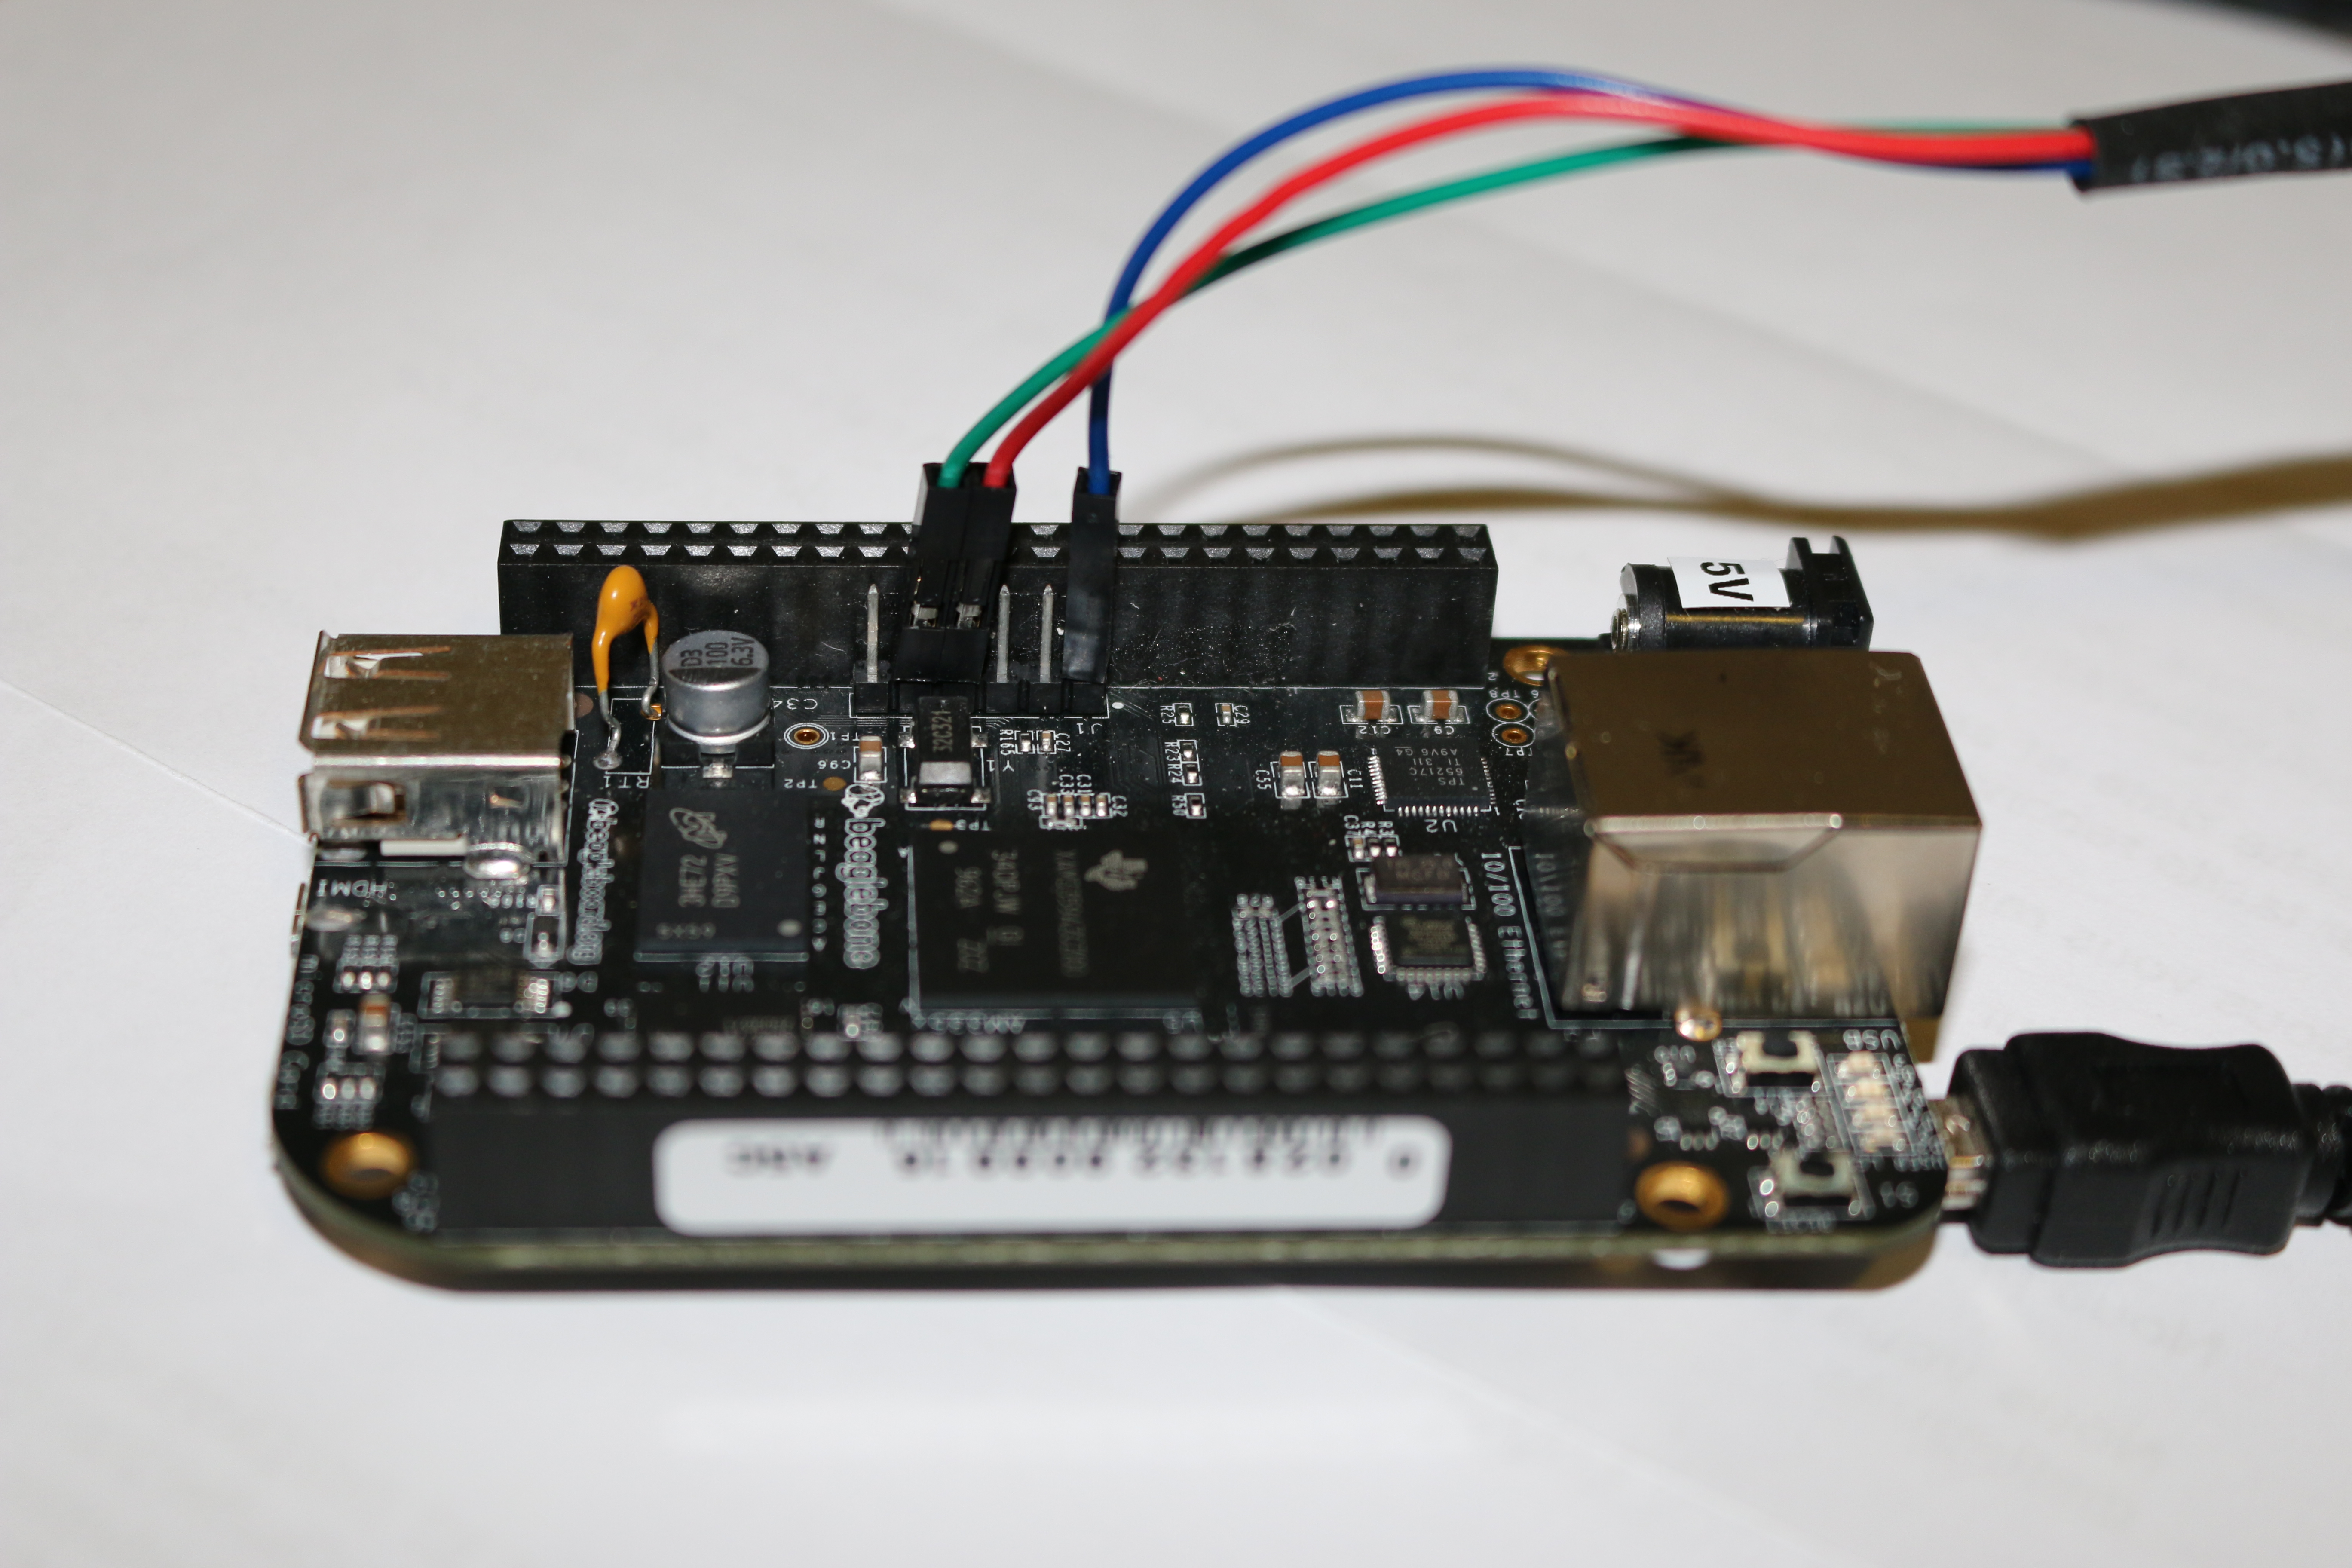
\includegraphics[width=8cm]{common/beaglebone-black-serial-connection.jpg}
\end{center}

Once the USB to Serial connector is plugged in, a new serial port
should appear: \code{/dev/ttyUSB0}.  You can also see this device
appear by looking at the output of \code{dmesg}.

To communicate with the board through the serial port, install a
serial communication program, such as \code{picocom}:

\begin{bashinput}
sudo apt install picocom
\end{bashinput}

If you run \code{ls -l /dev/ttyUSB0}, you can also see that only
\code{root} and users belonging to the \code{dialout} group have
read and write access to this file. Therefore, you need to add your user
to the \code{dialout} group:

\begin{bashinput}
sudo adduser $USER dialout
\end{bashinput}

{\bf Important}: for the group change to be effective, in Ubuntu 18.04, you have to
{\em completely reboot} the system \footnote{As explained on
\url{https://askubuntu.com/questions/1045993/after-adding-a-group-logoutlogin-is-not-enough-in-18-04/}.}.
A workaround is to run \code{newgrp dialout}, but it is not global.
You have to run it in each terminal.

Now, you can run \code{picocom -b 115200 /dev/ttyUSB0}, to start serial
communication on \code{/dev/ttyUSB0}, with a baudrate of \code{115200}. If
you wish to exit \code{picocom}, press \code{[Ctrl][a]} followed by
\code{[Ctrl][x]}.

Insert the SD card in the dedicated slot on the BeagleBone Black. Press the S2
push button (located just above the previous slot), plug in the USB cable and
release the push button. You should see boot messages on the console.

Wait until the login prompt, then enter \code{root} as user.
Congratulations! The board has booted and you now have a shell.

\section{Checking that we run a Patched kernel}

To check that we are indeed running a kernel with the preempt-RT patch applied and
full kernel preemption enabled, we have 2 main ways of checing.

First, use the \code{uname -a} command. Running an RT kernel should show the \code{PREEMPT_RT} version item.

The other way to check is to look at the file \code{/sys/kernel/realtime}. It's content is always '1', but the file only exists for RT kernels.

